%%%%%%%%%%%%%%%%%%%%%%%%%%% asme2e.tex %%%%%%%%%%%%%%%%%%%%%%%%%%%%%%%
% Template for producing ASME-format articles using LaTeX            %
% Written by   Harry H. Cheng                                        %
%              Integration Engineering Laboratory                    %
%              Department of Mechanical and Aeronautical Engineering %
%              University of California                              %
%              Davis, CA 95616                                       %
%              Tel: (530) 752-5020 (office)                          %
%                   (530) 752-1028 (lab)                             %
%              Fax: (530) 752-4158                                   %
%              Email: hhcheng@ucdavis.edu                            %
%              WWW:   http://iel.ucdavis.edu/people/cheng.html       %
%              May 7, 1994                                           %
% Modified: February 16, 2001 by Harry H. Cheng                      %
% Modified: January  01, 2003 by Geoffrey R. Shiflett                %
% Use at your own risk, send complaints to /dev/null                 %
%%%%%%%%%%%%%%%%%%%%%%%%%%%%%%%%%%%%%%%%%%%%%%%%%%%%%%%%%%%%%%%%%%%%%%

%%% use twocolumn and 10pt options with the asme2e format
\documentclass[twocolumn,10pt]{asme2e}
\special{papersize=8.5in,11in}
\usepackage{amsmath}
\usepackage{amsfonts}
\usepackage{relsize}
\usepackage{algorithm}
\usepackage{algpseudocode}
\usepackage{graphicx}
\usepackage{epsfig}
\usepackage{epstopdf}% To incorporate .eps illustrations using PDFLaTeX, etc.

%%%%%%%%%%%%%%%%%%%%%%%%%%%%%%%%%%%%%%%%%%%%%%%%%%%%%%%%%%%%%%%%%%%%%%%%%
%%%% Shorthands for greek letters %%%%%%%%%%%%%%%%%%%%%%%%%%%%%%%%%%%%%%%
%%%%%%%%%%%%%%%%%%%%%%%%%%%%%%%%%%%%%%%%%%%%%%%%%%%%%%%%%%%%%%%%%%%%%%%%%

% Command for generic OCP
%\newcommand{\fdyn}{\mathlarger{f}}
\newcommand{\Rnx}{\mathbb{R}^{n_{x}}} %R^nx mathematical set
\newcommand{\Rnu}{\mathbb{R}^{n_{u}}}
\newcommand{\Rng}{\mathbb{R}^{n_{g}}}
\newcommand{\Rnh}{\mathbb{R}^{n_{h}}}
\newcommand{\Rnr}{\mathbb{R}^{n_{r}}}


% Command for general collocation
\newcommand{\inset}[1]{\in [1,\dots,#1]}
\newcommand{\insetz}[1]{\in [0,\dots,#1]}
\newcommand{\pnh}{p_{n}h}
\newcommand{\hk}{h_{k}}                       % Discretization step 
\newcommand{\dkg}[1]{d_{k,#1}}                    % degree of i-state in k-interval
\newcommand{\dki}{d_{k,i}}                    % degree of i-state in k-interval
\newcommand{\dkip}{d_{k,i}^{+}}                    % degree of i-state in k-interval
\newcommand{\taudki}{\tau^{d_{k,i}}}     % Gauss-Legendre Collocation for i-state in k-interval
\newcommand{\bartaudki}{\bar{\tau}^{d_{k,i}}} % Collocation + tau = 0
\newcommand{\taujdki}{\tau_{j}^{d_{k,i}}}
\newcommand{\Tk}{T_{k}}                       % Time at k-grid-point 
\newcommand{\Tkjdki}{T_{k,j}^{d_{k,i}}}       % Time at j-collocation of i-state in k-interval 
\newcommand{\Xkidki}{X_{k,i}^{d_{k,i}}} % Lagrange poly for i-state in k-interval of degree dki 
\newcommand{\Lmdki}{L_{m}^{d_{k,i}}}
\newcommand{\xkim}{x_{k,i,m}}  
\newcommand{\xkpuu}[1]{x_{k+1,#1,1}}  
\newcommand{\xuuu}[1]{x_{1,#1,1}} 
\newcommand{\fdi}{f_{i}} 
\newcommand{\Vki}{V_{k,i}} 
\newcommand{\Xkd}{X_{k}^{d}}
\providecommand{\norm}[1]{\lVert#1\rVert}
\providecommand{\Xkdi}[1]{X_{k,#1}^{d_{k,#1}}}
\newcommand{\bardk}{\bar{d}_k}
\newcommand{\bardkm}{\bar{d}_k^{-}}
\newcommand{\lmbd}{l_{m}^{\bar{d}_{k}}}
\newcommand{\lmbdm}{l_{m}^{\bar{d}_{k}^{-}}}
\newcommand{\lmdki}{l_{m}^{d_{k,i}}}
\newcommand{\gkm}{g_{k,m}}
\newcommand{\taubardk}{\tau^{\bar{d}_{k}}}
\newcommand{\taudkip}{\tau^{{d}_{k,i}^{+}}}
\newcommand{\barXkidkip}{\bar{X}_{k,i}^{d_{k,i}^{+}}} 
\newcommand{\Ekij}{E_{k,i,j}}
\newcommand{\ekij}{e_{k,i,j}}
\newcommand{\dkis}{d_{k,i}^{*}}                    % degree of i-state in k-interval
\newcommand{\Bki}{B_{k,i}} 
\newcommand{\Pki}{P_{k,i}} 
\newcommand{\Dks}{D_{k}^{*}} 
\newcommand{\Dk}{D_{k}} 
\newcommand{\dksn}[1]{d_{k,#1}^{*}} 





%% The class has several options
%  onecolumn/twocolumn - format for one or two columns per page
%  10pt/11pt/12pt - use 10, 11, or 12 point font
%  oneside/twoside - format for oneside/twosided printing
%  final/draft - format for final/draft copy
%  cleanfoot - take out copyright info in footer leave page number
%  cleanhead - take out the conference banner on the title page
%  titlepage/notitlepage - put in titlepage or leave out titlepage
%
%% The default is oneside, onecolumn, 10pt, final

%%% Replace here with information related to your conference
\confshortname{IDETC/CIE 2022}
\conffullname{the ASME 2022 International Design Engineering Technical Conferences \&\\
              Computers and Information in Engineering Conference}

%%%%% for date in a single month, use
%\confdate{24-28}
%\confmonth{September}
%%%%% for date across two months, use
\confdate{August 14-17}
\confyear{2022}
\confcity{St. Louis, Missouri}
\confcountry{USA}

%%% Replace DETC2009/MESA-12345 with the number supplied to you
%%% by ASME for your paper.
\papernum{DETC2022/MSNDC-12345}

%%% You need to remove 'DRAFT: ' in the title for the final submitted version.
%\title{DRAFT: AN ARTICLE CREATED USING \LaTeX2\raisebox{-.3ex}{$\epsilon$}\ IN ASME FORMAT}
\title{A \MakeLowercase{$\pnh$}-adaptive refinement procedure\\
for numerical optimal control problems}
%%% for the discussion section only
%\usepackage{helvet}
%\title{\fontfamily{phv}\selectfont{\Huge{DRAFT: AN ARTICLE CREATED USING \LaTeX2\raisebox{-.3ex}{$\epsilon$}\ IN ASME FORMAT}}}

%%% first author
\author{Lorenzo Bartali\thanks{Address all correspondence to this author.}
    \affiliation{
	Dipartimento di Ingegneria Civile e Industriale\\
	Universit\`{a} di Pisa\\
	56122 Pisa PI, Italy\\
    Email: lorenzo.bartali@phd.unipi.it
    }	
}

%%% second author
%%% remove the following entry for single author papers
%%% add more entries for additional authors
\author{Marco Gabiccini\\
       {\tensfb Massimo Guiggiani}
    \affiliation{Dipartimento di Ingegneria Civile e Industriale\\
	Universit\`{a} di Pisa\\
	56122 Pisa PI, Italy\\
	Email: marco.gabiccini@unipi.it\\
\phantom{Email:} massimo.guiggiani@unipi.it
    }
}

\begin{document}

\maketitle

%%%%%%%%%%%%%%%%%%%%%%%%%%%%%%%%%%%%%%%%%%%%%%%%%%%%%%%%%%%%%%%%%%%%%%
\maketitle
%\begingroup
%\let\clearpage\relax


%%%%%%%%%%%%%%%%%%%%%%%%%%%%%%%%%%%%%%%%%%%%%%%%%%%%%%%%%%%%%%%%%%%%%%
\begin{abstract}
	{\it This paper presents an automatic procedure to enhance the accuracy of the numerical solution of an optimal control problem (OCP) discretized via direct collocation at Gauss-Legendre points. First, a numerical solution is obtained by solving a nonlinear program (NLP). Then, the method evaluates its accuracy and adaptively changes both the degree of the approximating polynomial within each mesh interval and the number of mesh intervals until a prescribed accuracy is met. %, thus following a ph-strategy.
The number of mesh intervals is increased for all state vector components alike, in a classical fashion. Instead, improving on state-of-the-art procedures, the degrees of the polynomials approximating the different components of the state vector are allowed to assume, in each finite element, distinct values. This explains the $\pnh$ definition, where $n$ is the state dimension. Instead, in the literature, the degree is always raised to the highest order for all the state components, with a clear waste of resources.
		%First, component-wise state error estimates are computed based on the difference between the Lagrange polynomial approximation and a corresponding estimate obtained by quadrature of the dynamics at Gauss-Legendre points within each finite element. Then, the derived error estimates are employed to establish whether the degree of the approximating polynomial should be increased or the mesh interval should be split into subintervals. The first option is selected if the degree suggested by the method remains below a given threshold for all state components. Otherwise, a finer mesh is created in those intervals where excessive error is registered. The NLP problem is solved again with the enhanced mesh and the evaluation procedure described is repeated. The process stops when a solution meets the specified error tolerance from the outset.
		
		Numerical tests on three OCP problems highlight that, under the same maximum allowable error, by independently selecting the degree of the polynomial for each state, our method effectively picks lower degrees for some of the states, thus reducing the overall number of variables in the NLP. Accordingly, various advantages are brought about, the most remarkable being: (i) an increased computational efficiency for the final enhanced mesh with solution accuracy still within the specified tolerance, (ii) a reduced risk of being trapped by local minima due to the reduced NLP size.}
\end{abstract} 

%%%%%%%%%%%%%%%%%%%%%%%%%%%%%%%%%%%%%%%%%%%%%%%%%%%%%%%%%%%%%%%%%%%%%%
\section*{INTRODUCTION}

Over the last three decades, direct collocation methods have become popular for the numerical solution of nonlinear optimal control problems, see e.g.,~\cite{Fahroo:JGCD:2002,Elnager:TAC:1995,Fahroo:JAS:2000,Gong:AAS:2006}, to mention only a few. In direct collocation methods, state and control functions are discretized at a set of appropriately chosen points in the time horizon considered. Then, the continuous time optimal control problem (OCP) is \emph{transcribed} to a finite-dimensional nonlinear program (NLP), and the NLP is coded and solved using different available software packages, such as~\cite{casadi:MPC:2019, Rao:TMS:2010,GPOPSII:TMS:2013}, typically interfaced with Interior-Point~\cite{Biegler:CCE:2009} or SQP~\cite{SNOPT:SIAMReview:2005} back-end solvers.

A rich variety of approaches has been proposed to obtain highly accurate solutions. A na\"{i}ve approach would be to resort to the use of high-resolution (dense) discretization grids, with a requirement of a large amount of CPU and memory resources, especially if the resulting NLP is not sparse. Solutions to reduce the computational burden associated to uniform grid discretizations have been proposed in~\cite{Betts:JCAM:2000}, where new grid points are introduced by solving an integer programming problem that minimizes the
maximum discretization error by subdividing the current grid. In~\cite{Ross:AAS:2003}, the pseudospectral knotting method, initially proposed in~\cite{Fahroo:ASC:2000}, has been generalized by exchanging information across the patches in the form of event conditions associated with the optimal control problem. In~\cite{Gong:AAS:2006}, the user specifies the number of nodes to be increased within a particular phase, in case the error of the computed optimal control between two successive iterations is
greater than a prescribed threshold. Here, the
gradient of the control is employed to determine the location of
the knots. In~\cite{Binder:CCE:2000} and~\cite{Binder:TechRep:2000}, a wavelet-Galerkin approach is used to discretize the OCP into an NLP and a local error analysis of the states and a wavelet analysis of the
control profile decides whether to add or remove wavelet basis functions. When state and control path constraints are present, \cite{Schlegel:CCE:2005}  uses wavelet analysis of the control profile to determine the
regions that require refinement. 
With the specific objective to trade numerical accuracy for robustness and complexity for execution speed, multiresolution techniques have been proposed in \cite{Jain:CDC:2007,Jain:JGCD:2008} for application that are time-critical, such as onboard real-time guidance and during emergency maneuvers.

Recently, a great deal of research effort has been devoted to the class of Gauss quadrature orthogonal collocation methods~\cite{Elnager:TAC:1995,Fahroo:JGCD:2002,Garg:Automatica:2010,Darby:JSR:2011,Darby:OCAM:2011}. In these approaches, the state is typically approximated using a Lagrange polynomial where the support points are chosen as Gauss quadrature points. The most advanced employ either Gauss-Legendre, Gauss-Radau or Gauss-Lobatto points~\cite{Biegler:book:2010}. Gauss quadrature collocation methods have been originally implemented as p methods with a single interval for the whole time horizon. Convergence of these methods was achieved by increasing the degree of the approximating polynomial. Their converge rate is exponential for problems with smooth and well-behaved solutions~\cite{Canuto:book:1988,Fornberg:book:1996}. On the contrary, h methods, where convergence is sought by increasing the number of mesh intervals, work well for problems whose solutions are non smooth, since even a low-order polynomial approximation can capture \emph{wild} solution behaviors on an extremely fine mesh. However, their converge rate is slow for problems with smooth solutions as compared to p methods.

With the goal of getting the best of both worlds, hp methods have been developed. Originally they were introduced for solving PDEs~\cite{Babuska:CMAME:1990}, while more recently they have been applied to OCPs as well~\cite{Darby:OCAM:2011,Darby:JSR:2011}. However, these approaches have demonstrated to create a great deal of noise in the error estimate, thereby making them computationally intractable when high-accuracy solutions are desired. Furthermore, the error estimate defined for these methods does not take advantage of the exponential convergence rate of a Gaussian quadrature collocation method.
Monitoring the error only in the state vector, Patterson at al.~\cite{Patterson:OCAM:2015} proposed a new ph-mesh refinement method that is very computationally efficient, does not suffer from noisy error estimates in~\cite{Darby:JSR:2011}, and produces larger mesh intervals for a given accuracy tolerance when compared with traditional fixed-order h methods.

Motivated by the relative simple ideas behind~\cite{Patterson:OCAM:2015}, in this paper we present an automatic procedure to enhance the accuracy of the numerical solution of an optimal control problem (OCP) discretized via direct collocation at Gauss-Legendre points. First, a numerical solution is obtained by solving an NLP with an initial uniform discretization. Then, the method evaluates its accuracy and adaptively changes both the degree of the approximating polynomial within each mesh interval and the number of mesh intervals until a prescribed accuracy is met, thus following the ph strategy proposed in~\cite{Patterson:OCAM:2015}.
The number of mesh intervals is increased concurrently for all state vector components, in a classical fashion. Instead, generalizing the procedure in~\cite{Patterson:OCAM:2015}, we present an algorithm that allows the degree of the approximating polynomial to assume distinct values for each state vector component and for each finite element. To the best of the authors' knowledge, in the research works found in literature, the degree is always raised to the highest order for all the state components, with an associated waste of computational resources and no practical accuracy benefit.
		The procedure prsented unfolds in two main steps: (i) component-wise state error estimates are computed based on the difference between the Lagrange polynomial approximation and a corresponding estimate obtained by quadrature of the dynamics at Gauss-Legendre points within each finite element; then, (ii) the derived error estimates are employed to establish whether (a) the degree of the approximating polynomial should be increased or (b) the mesh interval should be split into subintervals. Option (a) is selected if the degree suggested by the method remains below a given threshold for all state components. Otherwise, according to option (b), a finer mesh is created in those intervals where excessive error is registered.
The NLP problem is solved again with the enhanced mesh and the evaluation procedure described is repeated. The process stops when, with the refined mesh and degree, the NLP solution meets the prescribed error tolerance from the outset.

To foster the generalization proposed, we analyze its numerical results on three OCP problems. The mesh refinement outcomes highlight that, given a maximum error threshold, by allowing to select the increase in the approximating polynomial degree independently for each state, our method effectively chooses to raise them frugally, this reducing the overall number of NLP variables needed with clear benefits in terms of reduced CPU time, memory usage and reduced risk of being trapped in local minima.



%%%%%%%%%%%%%%%%%%%%%%%%%%%%%%%%%%%%%%%%%%%%%%%%%%%%%%%%%%%%%%%%%%%%%%
\section*{OPTIMAL CONTROL PROBLEM}

In this work, the $\pnh$ adaptive refinement algorithm is applied to a general optimal control problem (OCP). Therefore, with the aim to introduced the notation used in the rest of the paper, in this section the overall structure of an OCP and its main components are briefly recalled.


The general form of an OCP can be written as
%\begin{equation}\label{OCP}
%	\begin{split}
%		&\underset{X,U}{\text{minimize}}\hspace{8mm} J = \int_{0}^{T}l(X(t),U(t))\,dt + E(X(T))\\
%		&\begin{split}
%			\text{subject to} \hspace{8mm} & \dot{X} -  f(X(t),U(t))			= 0, \hspace{5mm} t \in[0,T]\\
%			& h(X(t),U(t)) \leq 0,  \hspace{11.5mm} t \in[0,T]\\
%			& r(X(T),U(T)) \leq 0,
%		\end{split}		
%	\end{split}
%\end{equation}
\begin{subequations}\label{OCP}
	\begin{align}
	\underset{X,U}{\text{minimize}}\hspace{8mm} &J = \int_{0}^{T}g(X(t),U(t))\,dt + E(X(T)) \label{eq:cost}\\
	\text{subject to} \hspace{8mm} &\dot{X}(t) -  f(X(t),U(t)) = 0, \hspace{5mm} t \in[0,T] \label{eq:dyn}\\
	& h(X(t),U(t)) \leq 0,  \hspace{11.5mm} t \in[0,T] \label{eq:path}\\
	& r(X(T),U(T)) \leq 0, \label{eq:terminal}		
	\end{align}
\end{subequations}

where $t$ is the independent variable (time), $T$ is the terminal time, $X \in \Rnx$ and $U \in \Rnu$ are the states and the controls, respectively, and $f (\cdot)$ is the dynamic vector field.

The OCP is characterized by an integral cost function, with a running cost $g$, a terminal cost $E(X(T))$, and three kinds of constraints: dynamics $\dot{X}-f(\cdot) \in \Rnx$, inequality $h(\cdot) \in \Rnh$, and terminal constraints $r(\cdot) \in \Rnr$.
The solution of the OCP  consists of the controls $U^{*}(t)$ and the states $X^*(t)$  minimizing the integral cost function while satisfying the above constraints.




%%%%%%%%%%%%%%%%%%%%%%%%%%%%%%%%%%%%%%%%%%%%%%%%%%%%%%%%%%%%%%%%%%%%%%
\section*{LEGENDRE-GAUSS COLLOCATION METHOD WITH TAILORED STATE DEGREES}
The %$\pnh$ form of the
continuous optimal control problem introduced in the previous section is discretized using the \emph{direct collocation} method at Gauss-Legendre collocation points. As a consequence, the original OCP becomes a \emph{Nonlinear Program} (NLP). In \emph{direct collocation} method the time horizon is discretized on a fixed mesh, where the generic interval is denoted as $S_{k} = [T_{k-1}, T_{k}]$, with mesh step $h_{k} = T_{k-1} - T_{k}$ ($k = 1, \ldots, N $). The values at mesh points (nodal values) are indicated by $X_{k}$, $U_{k}$ and $T_{k}$, for  states, controls and time, respectively.
The parametrization of the controls on the same mesh is chosen as piecewise constant, which yields to a constant control $U(t) = U_{k}$ on each interval $S_k$.

As far as states in $S_{k}$ are concerned, classical approaches appearing in the literature approximate all of them by polynomials of the same degree $d$.
Instead, in this paper we can pick different degrees for each state and for each mesh interval. Hence, the $i$-th state component on the $S_{k}$ subinterval is approximated by a polynomial of degree $\dki$ defined as follows
\begin{subequations}
	\begin{align}
	&\Xkidki (\tau) = \sum_{m=1}^{\dkip} \Lmdki(\tau)\xkim, \hspace{5mm} \text{with} \label{Xpoly}\\
	&\Lmdki (\tau) = \prod_{r=1, r\neq m}^{\dkip} \dfrac{\tau - \bartaudki_{r}}{\bartaudki_{m} - \bartaudki_{r}}, \label{BLagrange}
	\end{align}
\end{subequations}
where $\dkip = \dki + 1$, $\tau \in [0,1]$ is the normalized time on $S_k$ such that $T_k(\tau) = T_{k-1} + h_k\tau$.
Basis functions $\Lmdki (\tau)$ are the Lagrange polynomials of degree $\dki$, calculated considering the points $\bartaudki = [\tau_{0}, \taudki]$, where $\tau_{0} = 0$ and $\taudki$ are the $\dki$ Gauss-Legendre collocation points. In our notation, $\taudki$  represents the vector of collocation points and $\bartaudki$ represents its \emph{augmented} version obtained by appending $\tau_{0}$ in the first position.
Then, $\bartaudki_{j}$ indicates the $j$-th component of $\bartaudki$ vector.
Finally, $\xkim$ is the values of the $i$-th state polynomial in interval $S_k$ at $\bartaudki_{m}$.

In order to apply collocation equations, ensuring that the system dynamics is satisfied at discrete points, the derivative of the generic polynomial $\Xkidki (\tau)$ comes into play. This is defined as
\begin{equation}
\Vki (\tau) = \frac{d}{d\tau}\Big(\Xkidki(\tau)\Big) = \sum_{m=1}^{\dkip}\Big(\frac{d}{d\tau}\Lmdki(\tau)\Big)\xkim
\end{equation}
Moreover, it is useful to define quantity $\Xkd (\tau)$ as
\begin{equation}
\Xkd(\tau) =
\begin{bmatrix}
\Xkdi{1}(\tau),\, \cdots \, \Xkdi{i}(\tau), \, \cdots\,
\Xkdi{n_x}(\tau)
\end{bmatrix}^T
\end{equation}
which represents, in the generic interval $S_k$ and for a given $\tau$, the evaluation of all state polynomials each of its own degree ($\dkg{1}, \dots, \dkg{i}, \dots, \dkg{n_{x}}$).

In \emph{direct collocation} Eqn.~(\ref{eq:dyn}), for the $i$-th state on the $k$-th interval, reads as
\begin{equation}\label{eq:colloc}
\Vki \left(\taujdki \right) = f_i\left(\Xkd \left(\taujdki\right),  U_k\right)\, \hk, \hspace{5mm} j = 1, \dots, \dki
\end{equation}
where $\taujdki$ is the $j$-th collocation point for the $i$-th state and $f_i(\cdot)$ is the $i$-th component of the vector field representing system dynamics. Eqns.~\eqref{eq:colloc} have to be imposed for all state components ($i = 1, \dots, n_x$) and for all mesh interval ($k = 1, \dots, N$).

To completely define the state polynomial, it is necessary to add the continuity equations  as equality constraint of the resulting NLP as follows
\begin{equation}\label{eq:continuity}
\Xkd(1) - X_k = 0, \hspace{5mm} k = 1, \dots, N-1
\end{equation}
where the nodal values of the state are linked to the $\xkim$ by the following equation
\begin{equation}
X_k = [\xkpuu{1}, \dots, \xkpuu{i}, \dots, \xkpuu{n_{x}}], \hspace{5mm} k = 1, \dots, N-1
\end{equation}
For $k = 1$ and $k = N$, the following boundaries conditions are imposed
\begin{align}
	X_{0}         &= \bar{X}_{0} \label{eq:intial},\\
	X_{N}^{d}(1)  &= X_N \label{eq:final},
\end{align}

where $X_0 = X(0) = [\xuuu{1}, \dots, \xuuu{i}, \dots, \xuuu{n_{x}}]$, $\bar{X}_{0}$ is an assigned initial value and $X_{N} = X(T)$ is the final nodal value.


The generic path constraint of Eqn.~(\ref{eq:path}), for each $S_k$, becomes
\begin{equation}\label{eq:nlpath}
h(X_k, U_k) \leq 0. \hspace{5mm} k = 1, \dots, N
\end{equation}

Then, the terminal constraints of Eqn.~(\ref{eq:terminal}) is
\begin{equation}\label{eq:npterminal}
	r(X_N, U_N) \leq 0. \hspace{5mm}
\end{equation}

As regards the cost function, the integral of Eqn.~(\ref{eq:cost}) is numerically approximated with a quadrature scheme that employs, for each interval, the collocation points associated to the state components with the highest degree. In such manner, the best integral approximation is guaranteed. Hence, the running cost $g(t)$ in the $S_k$ interval can be rewritten as
\begin{subequations}
	\begin{align}
	& g_k(\tau) = \sum_{m=1}^{\bardk} \lmbdm(\tau)\gkm, \hspace{5mm} \text{with} \label{eq:nlpcost}\\
	&  \lmbdm (\tau) = \prod_{r=1, r\neq m}^{\bardk} \dfrac{\tau - \taubardk_{r}}{\taubardk_{m} - \taubardk_{r}}, \label{eq:nlplm}
	\end{align}
\end{subequations}
where $\bardk = \max\limits_{i= 1, \dots, n_x}(\dki)$, $\bardkm = \bardk -1$, $\lmbdm$ are the Lagrange polynomials of degree $\bardkm$, $\taubardk$ are the $\bardk$ Gauss-Legendre collocation points, and $\gkm$ is the value of $g_k (\tau)$ at $\taubardk_{m}$.

From this polynomial approximation the numerical integral $J_k$ of the running cost function $g(t)$ in the $k$-th element can be obtained from the following equation
\begin{equation}\label{eq:nlpcostk}
	J_k = \sum_{m=1}^{\bardk}\Big(\int_{0}^{1}\lmbd(\tau)d\tau\Big)\gkm \hk.
\end{equation}
With the equations shown in this section it is possible to transform the original OCP into an NLP by writing them for $k = 1, \dots, N$, and considering that the total cost function $J$, that has to be minimized, is given by $J = \sum_{k=1}^{N}J_k$.

It is worth noting that, unlike~\cite{Patterson:OCAM:2015} where the dynamics is collocated using the \emph{implicit integral form}, here the \emph{differential form} is used.
Furthermore, even if the collocation method was generalized by using a different degree for the polynomial approximation of $i$-th state on the $k$-th mesh interval, by choosing a degree $d$ in a way that $\dki = d$, for $i = 1, \dots, n_x$ and $k = 1, \dots, N$, the classical collocation method can be implemented.


%%%%%%%%%%%%%%%%%%%%%%%%%%%%%%%%%%%%%%%%%%%%%%%%%%%%%%%%%%%%%%%%%%%%%%
\section*{$p_n h$-ADAPTIVE MESH REFINEMENT METHOD}

In this section a $\pnh$-adaptive mesh refinement method is developed. In particular, the generic OCP problem is first transcribed into an NLP using the \emph{direct collocation} method, explained above, then the mesh refinement method is applied to the obtained optimal solution.
The $\pnh$ method explained here is closely related to~\cite{Patterson:OCAM:2015}. In particular, the method for estimating the error in the current solution is adapted from the aforementioned reference. The key novelty here is the refinement strategy.
In~\cite{Patterson:OCAM:2015}, the adjustment of the polynomial degree is perfomed such that all states are represented by the same degree. Instead, in this work, the $p$-refinement is different for each state. Instead, similarly to~\cite{Patterson:OCAM:2015}, the mesh spacing is adjusted only if the approach to reach convergence by solely increasing the polynomial degree fails.


%%%%%%%%%%%%%%%%%%%%%%%%%%%%%%%%%%%%%%%%%%%%%%%%%%%%%%%%%%%%%%%%%%%%%%
\subsection*{Error Estimate}

In this section, an estimate of the relative error in the solution within a mesh interval is derived. The error is calculated in each mesh interval, for each state.
The key idea is to compare the optimal state obtained from the NLP solution, with a more accurate approximation of the state.

To explain in details this aspect, consider the $i$-th state on the generic $S_k$ mesh interval.
The solution of NLP gives as output a polynomial approximation of the state, that has been called $\Xkidki (\tau)$.
If the problem solution is suppose to be smooth, a polynomial approximation obtained with an increase number of Gauss-Legendre points should yield a state that more accurately satisfies the dynamics.
Suppose that the error has to be estimated at a set of  $\dkip = \dki + 1$ collocation points, that consistent whit the proposed notation are indicated by $\taudkip$.
The values of the NLP solution in these points are denoted by $\Xkidki (\taudkip_j)$ for $j = 1, \dots, \dkip$.
Then the improved approximation of the state is constructed by using the value of the right-hand side of the dynamics at these new Gauss-Legendre points.
Let $\barXkidkip (\tau)$ be a polynomial of degree $\dkip$ that is defined for the $i$-th state on the $S_k$ interval. If the derivative of this polynomial matches the dynamics at each $\taudkip$ collocation points, $\barXkidkip (\tau)$ can be obtained by a numerical integration using the resulting quadrature scheme

\begin{subequations}
\begin{align}
	&\barXkidkip (\tau) = \sum_{m=1}^{\dkip}\Big(\int_{0}^{\tau}\lmdki (\tau)d\tau\Big) f_i\Big(\Xkd(\taudkip_m), U_k\Big), \hspace{2mm} \text{where} \label{eq:barX}\\
	&  \lmdki (\tau) = \prod_{r=1, r\neq m}^{\dkip} \dfrac{\tau - \taudkip_r}{\taudkip_m - \taudkip_r}. \label{eq:meshlm}
\end{align}

\end{subequations}

Hence $\barXkidkip (\tau)$ represents the improved approximation and its values in $\taudkip$ will be denoted by $\barXkidkip (\taudkip_j)$ for $j = 1, \dots, \dkip$.

Defined these quantities it is possible to evaluate the absolute and relative errors for each $\taudkip_j$ of the $i$-th state on the $k$-th interval

\begin{subequations}
	\begin{align}
	&\Ekij = \Big|\barXkidkip (\taudkip_j) - \Xkidki (\taudkip_j)\Big| \label{eq:absolute}\\
	&\ekij = \dfrac{\Ekij}{1 + \max\limits_{j= 1, \dots, \dkip} \Big| \Xkidki (\taudkip_j)\Big|} \label{eq:relative}
	\end{align}
\end{subequations}

where Eqn.~(\ref{eq:absolute}) and Eqn.~(\ref{eq:relative}) are the absolute and the relative error in the $\taudkip_j$, respectively.

The relative error is use in the next section to implement the $\pnh$ strategy.

%%%%%%%%%%%%%%%%%%%%%%%%%%%%%%%%%%%%%%%%%%%%%%%%%%%%%%%%%%%%%%%%%%%%%%
\subsection*{Algorithm}
In this section the algorithm implemented for mesh refining is shown.
Suppose further that it is desired to meet a relative error accuracy tolerance $\epsilon$ in each mesh
interval $S_k$ for $k = 1, \dots, N$. If the tolerance  $\epsilon$  is not met in at least one mesh interval, then the next step is to refine the current mesh, either by dividing the mesh interval or increasing the degree of the approximating polynomial within the mesh interval.
In particular, to make it clearer, the method is shown in a pseudocode form and for the generic $S_k$ mesh interval.
To better understand the pseudocode, it is worth to explain some quantities that appear in it.
Hence, $\dkis$ is the new polynomial degree that has to be chosen, for the $i$-th state in the $S_k$ interval, to reach the prescribed tolerance $\epsilon$. Then $\Bki$ is the number of subinterval into which $S_k$ has to be divided, to respect $\epsilon$, considering the error of the $i$-th state. If $\Bki = 1$, $S_k$ has not to be divided . Instead $d_{min}$ and $d_{max}$ are the maximum and the minimum allowable polynomial degree.

%% Definire dmax, dmin, Bki, d*, epsilon



\begin{algorithm}
\caption{Exploration: Step 1 of the $\pnh$ mesh refinement}\label{alg:step1}
	\begin{algorithmic}[1]
		\For {$i = 1$ to $n_x$}
			\If{$\max\limits_{j= 1, \dots, \dkip} (\ekij) \leq \epsilon$}
				\State $\dkis \gets \dki$
				\State $\Bki \gets 1$  %\Comment{This is a comment}
			\Else
				\State $\Pki \gets \log_{\dki} \Bigg\lceil \max\limits_{j= 1, \dots, \dkip} \Bigg(\dfrac{\ekij}{\epsilon}\Bigg) \Bigg\rceil$
				\State $\dkis \gets \dki + \Pki$
					\If {$ \dkis \leq d_{max}$}
						\State $\Bki \gets 1$		
					\Else
						\State $\Bki \gets \max\Bigg(\Bigg\lceil \dfrac{\dkis}{d_{min}}\Bigg\rceil, 2\Bigg)$
					\EndIf
			\EndIf
		\EndFor
	\end{algorithmic}
\end{algorithm}

In Alg.~\ref{alg:step1} the first step of the proposed refine method is explained. In particular, the quantity $P_{k,i}$ is calculated referring to the method of~\cite{Patterson:OCAM:2015} which is in accordance with the convergence theory summarized in~\cite{Hou:GNC:2012,Hou:PHD:2013}.  After Alg.~\ref{alg:step1} two vectorial quantities are defined $\Dks = [\dksn{1}, \dots, \dksn{i}, \dots, \dksn{n_x}]$ and $\Dk = [\dkg{1}, \dots, \dkg{i}, \dots, \dkg{n_x}]$. Then the refinement step, shown in Alg.~\ref{alg:step2} is performed.

\begin{algorithm}
	\caption{Refinement: Step 2 of the $\pnh$ mesh refinement}\label{alg:step2}
	\begin{algorithmic}[1]
		\If {$\max\limits_{i= 1, \dots, n_x}(\Bki) = 1$}
			\If {$\Dks = \Dk$}
				\State stop algorithm, convergence reached	
			\Else
				\For {$i = 1$ to $n_x$}
					\State $\dki = \dkis$ \Comment p-refinement
				\EndFor
			\EndIf
		\Else
			\For {$i = 1$ to $n_x$}
				\State $\dki = \dki$
				\State $\Bki = \max\limits_{i= 1, \dots, n_x}(\Bki)$ \Comment h-refinement
			\EndFor		
		\EndIf
	\end{algorithmic}
\end{algorithm}


The new mesh for the next NLP, is encoded in the quantity $\dki$ and $\Bki$ for $i = 1, \dots, n_x$ and for $k = 1, \dots, N$.

It is worth to notice that, as explained in Alg.~\ref{alg:step2}, in each interval, if at least one of the state required to split $S_k$, then it is splitted. Instead if no state required it, each state is approximated, in the next NLP, with a polynomial of degree equal to the one proposed by the method.

Finally, the proposed algorithm can match the original mesh refinement method of~\cite{Patterson:OCAM:2015} with two simple steps: (i) The first NLP has to be solved in a way that all the states have the same degree $d_k$ in $S_k$, therefore $\dki = d_k$ (for $i = 1, \dots, n_x$), (ii) The $6$-th line of Alg.~\ref{alg:step2} has to be modified by writing $\dki = \max\limits_{i= 1, \dots, n_x}(\dkis)$. In this way the polynomial approximation maintains always the same degree for all the states.





%%%%%%%%%%%%%%%%%%%%%%%%%%%%%%%%%%%%%%%%%%%%%%%%%%%%%%%%%%%%%%%%%%%%%%
\section*{EXAMPLES}
In this section, three different examples are discussed. Their purpose is to numerically showcase that our method allows to adaptively refine the mesh to accurately solve an OCP, similarly to ~\cite{Patterson:OCAM:2015}, with the remarkable advantage of an increased computational efficiency for the final enhanced mesh without hindering the accuracy of the final solution. 
%still within the specified tolerance. 
In fact, by allowing to increase the degrees of the approximating polynomials independently for each state, our method effectively adopts to raise them carefully and in a tailored manner. This allows to reduce the overall number of variables of the resulting NLP, with clear benefits in terms of reduced CPU time, memory usage and reduced risk of being trapped by local minima.

Let us now direct our attention to the details. Each problem is transcribed in its initial NLP version by choosing $N = 20$ mesh intervals and by assigning a degree $\dki = 2$ everywhere, i.e. for all $i = 1, \dots, n_x$ and  $k = 1, \dots, N$. The mesh refinement algorithm is then applied with $d_{\min} = 2$, $d_{\max} = 8$ with a prescribed maximum allowable relative error $\epsilon = 1 \cdot 10^{-3}$.

It is worth observing that the $p_{n}h$ tag and the $ph$ tag indicate our mesh refinement method and the one originally proposed by Patterson et al.~\cite{Patterson:OCAM:2015}, respectively.

It is also worth remarking that the final refined mesh for all the three presented examples (both in terms of number and size of $S_{k}$ intervals), turns out to be the same by rolling out both the $p_{n}h$ and the $ph$ approaches. This arises partly as a result that algorithms share the last section (lines 9-14) of the \emph{Execution} pass in {\bf Algorithm~\ref{alg:step2}}. This means the generic $S_k$ interval is subdivided if and only if at least one state in the generic $S_k$ asks for it.

Each transcribed optimal control problem is coded in a scripting environment using the \texttt{MATLAB} interface to the open-source CasADi framework~\cite{casadi:MPC:2019}. 
The CasADi suite can perform AD (automatic differentiation) on the code to compute gradients and Jacobians and provides building blocks to efficiently formulate and solve large-scale optimization problems. The back-end solver adopted is IPOPT~\cite{Biegler:CCE:2009} which implements an interior-point algorithm. All the associated NLPs are solved on a laptop with 2.30GHz Intel(R) Core(TM) i7-10875H CPU and 32 GB of RAM.



%%%%%%%%%%%%%%%%%%%%%%%%%%%%%%%%%%%%%%%%%%%%%%%%%%%%%%%%%%%%%%%%%%%%%%
\subsection*{Van Der Pol}
Considering the following optimal control problem namely
driving a \emph{Van der Pol} oscillator to the origin, taken from reference~\cite{casadi:DOC:2018},

\begin{subequations}\label{eq:vanderpol}
	\begin{align}
	\underset{X \in \mathbb{R}^{2}, \, U \in \mathbb{R}}{\text{minimize}}\hspace{8mm}
	&J = \int_{0}^{T}(x_1^{2} + x_2^{2} + u^{2})\,dt  \label{eq:vancost}\\
	\text{subject to} \hspace{8mm}
	& \dot{x}_1 = (1 - x_2^{2})x_{1} - x_2 + u \hspace{5mm} t \in[0,T] \label{eq:vandyn1}\\
	& \dot{x}_2 = x_1 \hspace{28.5mm} t \in[0,T] \label{eq:vandyn2}\\
	& -1  \leq u \leq 1,  \hspace{20mm} t \in[0,T] \label{eq:vanpath1}\\
	& x_2 \geq -0.25,  \hspace{21.5mm} t \in[0,T] \label{eq:vanpath2}\\
	& x_1(0) = 0, \label{eq:initial1}\\		
	& x_2(0) = 1, \label{eq:intial2}		
	\end{align}
\end{subequations}

where $x_1$ and $x_2$ are the two state component (hence $X(t) = [x_1(t), x_2(t)]$), $u$ indicates the element of $U$ (which has dimension $1$), and the dynamics constraints and the initial conditions have been shown explicitly for each state component. In particular, $\dot{X}(t) = [\dot{x}_1(t), \dot{x}_2(t)]$.

In Figs.~\ref{fig:pnh1vanderpol}-\ref{fig:pnh2vanderpol} is shown, for the $\pnh$ algorithm and for the $ph$ one, the final degree of the first state component ($x_1$) and of the second one ($x_2$), respectively. Comparing with the red line, which represents the initial degree, each method increases the states degree. In particular, the green line is equal for the two figures, this means that each state has always the same polynomial degree approximation. Instead, the blue ones are different, hence each state has a different final polynomial approximation. Furthermore, considering the original $S_k$ steps delimited by the dashed gray lines, observing where the green and blue markers increase, it is possible to notice where an $h$-strategy is adopted.
\begin{figure}
	\centering
	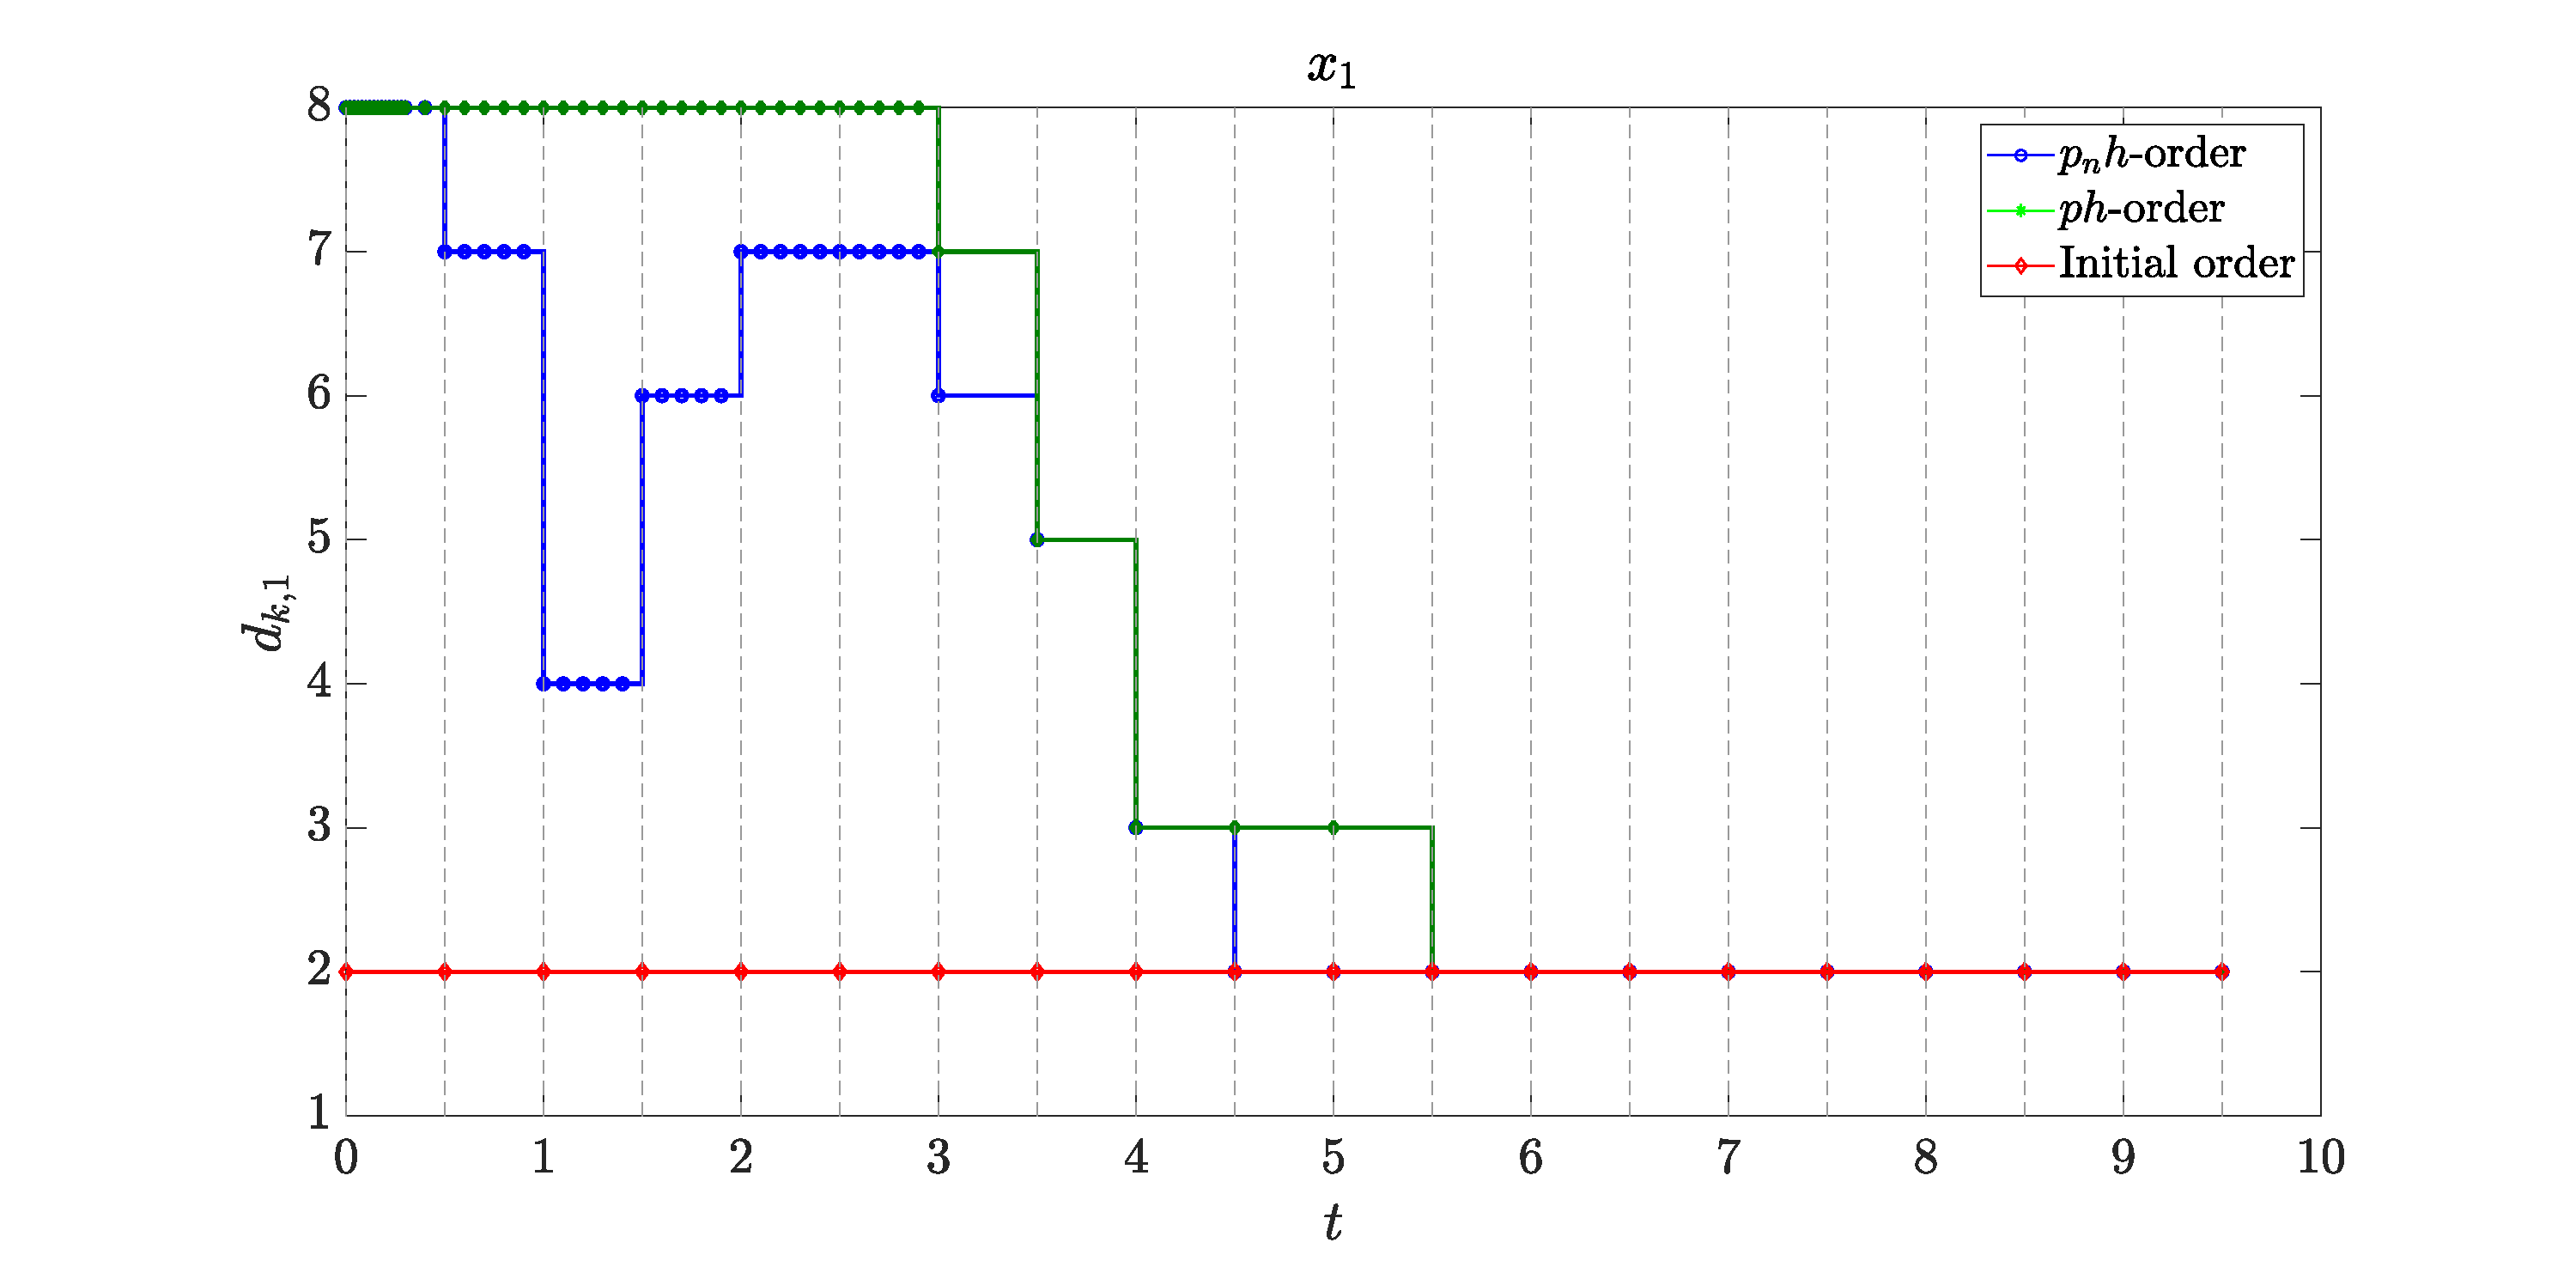
\includegraphics[trim={2cm 0cm 4cm 0cm},clip,width=1.\linewidth]{Img/pnh1_vanderpol}
	\caption{POLYNOMIAL DEGREE OF SECOND STATE ($x_{1}$) FOR THE INITIAL MESH (RED) $\pnh$ ALGORITHM (BLUE) AND $ph$ ALGORITHM (GREEN).}
	\label{fig:pnh1vanderpol}
\end{figure}

\begin{figure}
	\centering
	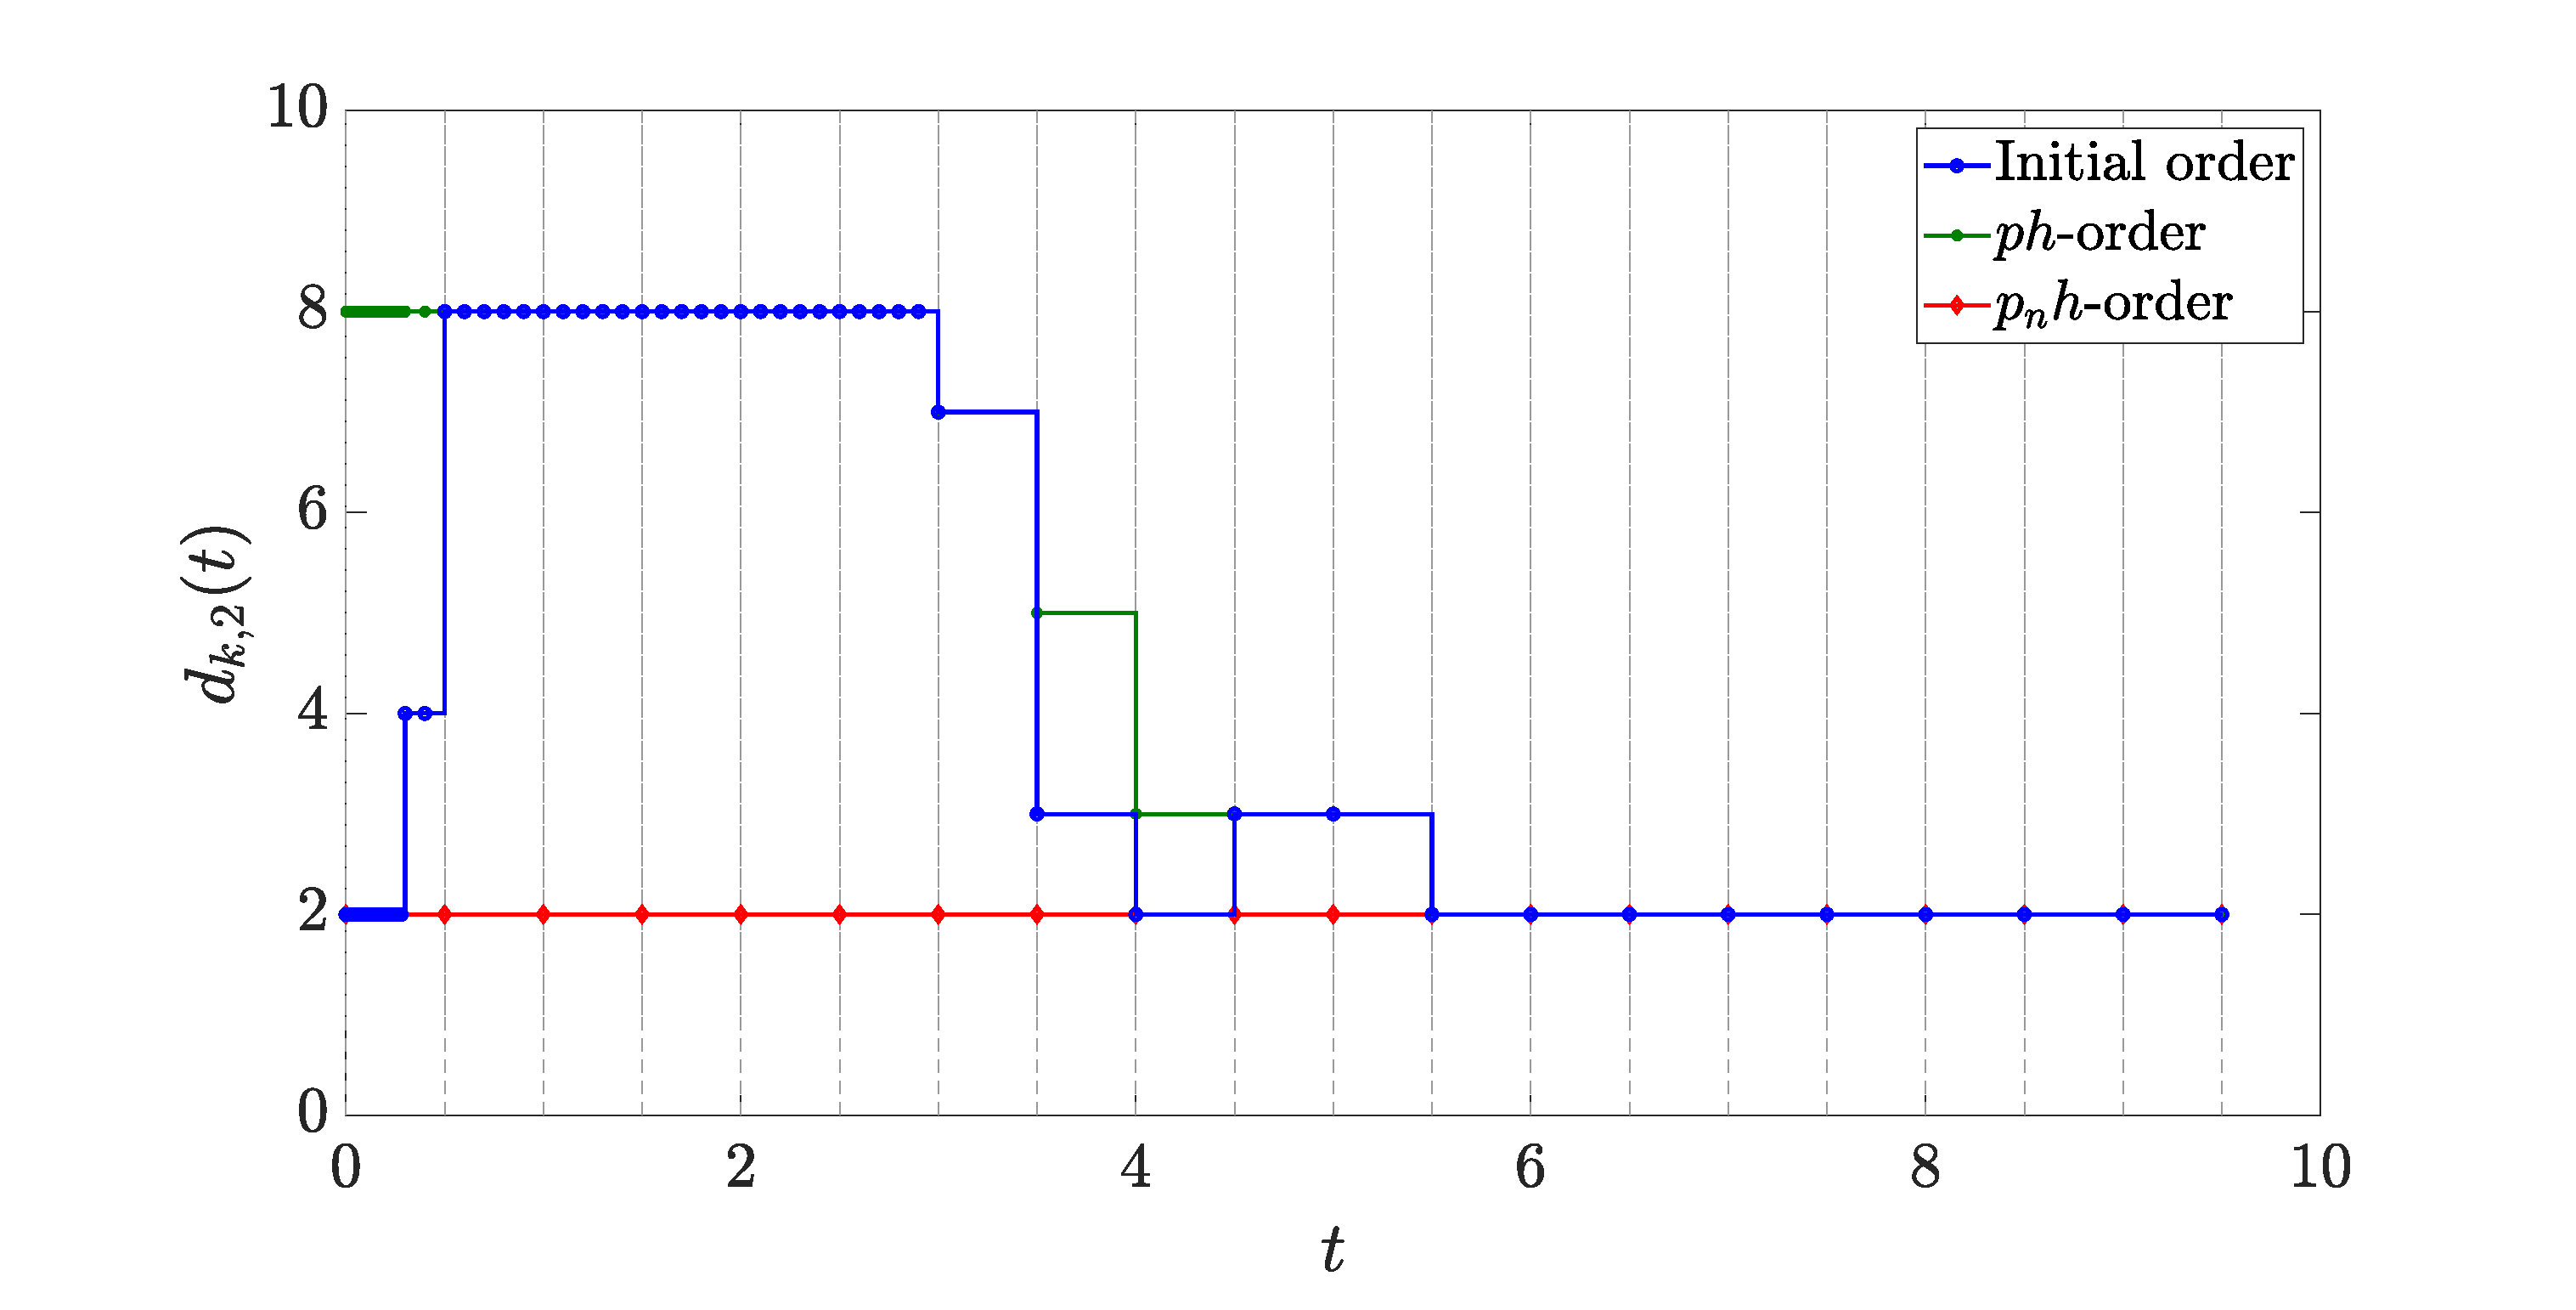
\includegraphics[trim={2cm 0cm 4cm 0cm},clip,width=1.\linewidth]{Img/pnh2_vanderpol}
	\caption{POLYNOMIAL DEGREE OF SECOND STATE ($x_{2}$) FOR THE INITIAL MESH (RED) $\pnh$ ALGORITHM (BLUE) AND $ph$ ALGORITHM (GREEN).}
	\label{fig:pnh2vanderpol}
\end{figure}

In Fig.~\ref{fig:vanderpolstates} the states profile obtained with the $\pnh$ final mesh is shown. In this case the dashed gray lines delimit the final $S_k$ interval. In particular, the nodal values are shown in blue, instead the collocation points in red. That figure shows clearly that the $\pnh$ mesh refinement method places many more collocation and mesh points where the states have greater variations.


\begin{figure}
	\centering
	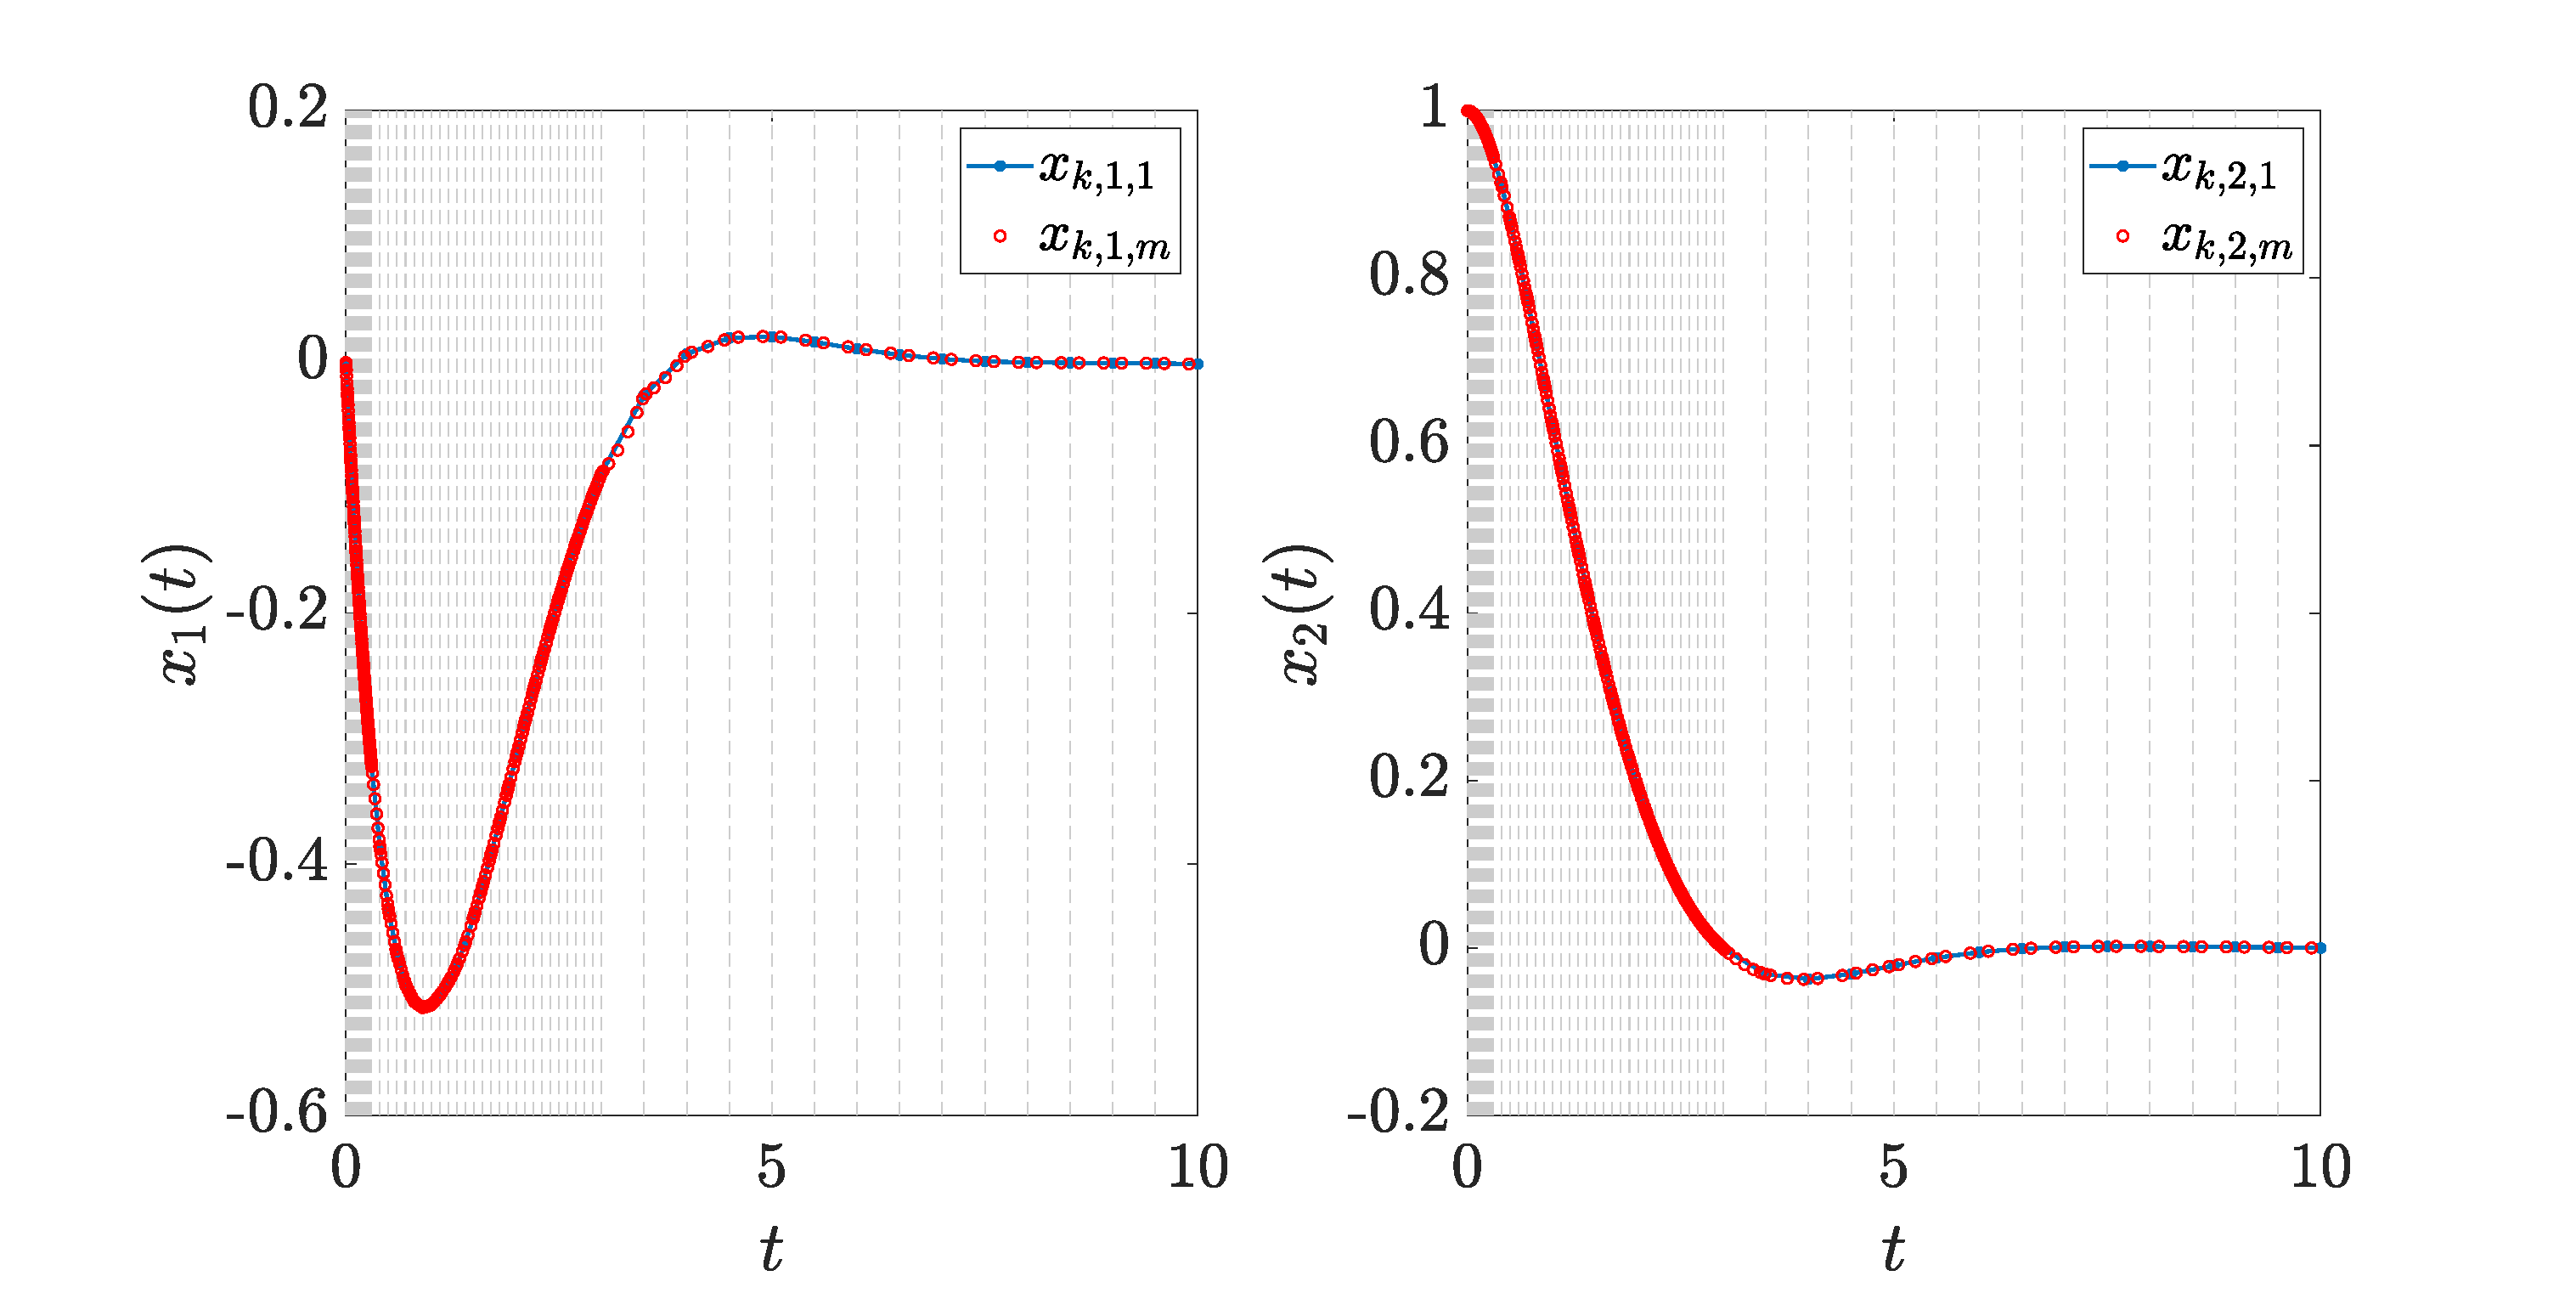
\includegraphics[trim={2cm 0cm 4cm 0cm},clip,width=1.\linewidth]{Img/vanderpol_states}
	\caption{OPTIMAL STATES PROFILE OBTAINED WITH THE $\pnh$ METHOD.}
	\label{fig:vanderpolstates}
\end{figure}

The advantages of the $\pnh$ method, respect to the $ph$ one, are shown in Tab.~\ref{tab:tablevanderpol}, where the column "Mesh" indicates the type of discretization mesh, in particular, "Initial" refers to the initial mesh problem and $ph$ and $\pnh$ refers to the final mesh (hence, the one which guarantees the respect of the $\epsilon$ tolerance), of the~\cite{Patterson:OCAM:2015} and our method, respectively. Then "NLP V." indicates the NLP variables of the resulting discretized OCP problem, "Time NLP" indicates the necessary time to solve the optimal control problem, and "N.I." refers to the number of algorithm iteration necessary to reach the given tolerance. Finally, "Time tot." refers to the total CPU time necessary to reach the imposed convergence criterion, and $e_{max}$  is the maximum of the local error $\ekij$, hence

\begin{equation}
e_{max}= \max\limits_{\substack{j = 1, \dots, \dkip \\ i = 1, \dots, n_x \\ k = 1, \dots, N}} (\ekij)
\end{equation}

\begin{table}[h]
	\caption{FUNDAMENTAL RESULTS QUANTITIES}
	\begin{center}
		\label{tab:tablevanderpol}
		\begin{tabular}{c l l l c c c}
			& & \\ % put some space after the caption
			\hline
			Mesh & NLP V. & Time NLP & N.I. & Time tot. & $e_{max}$ \\
			\hline
			Initial & 140 & 138ms & / & / &  $3.7\mathrm{e}{-2}$\\
			$ph$ & 918 & 500ms & 4 & 23.1s & $9.1\mathrm{e}{-4}$ \\
			$\pnh$ & 769 & 400ms & 4 & 19s & $9.5\mathrm{e}{-4}$ \\
			\hline
		\end{tabular}
	\end{center}
\end{table}

It is worth noting that $\pnh$ method leads to an optimal solution that while respecting the given tolerance $\epsilon$, is obtained from an NLP with fewer variables than $ph$ algorithm.
Hence the final NLP obtained from $\pnh$ method required a lower computational cost and a shorter CPU time.

!!!Figure %%Furthermore considering that $ph$ and $\pnh$ have the same final mesh in terms of $S_k$ number and size, by comparing the solution at the nodal values, the maximum difference between the two solution is for the optimal control $u$.............

\begin{figure}
	\centering
	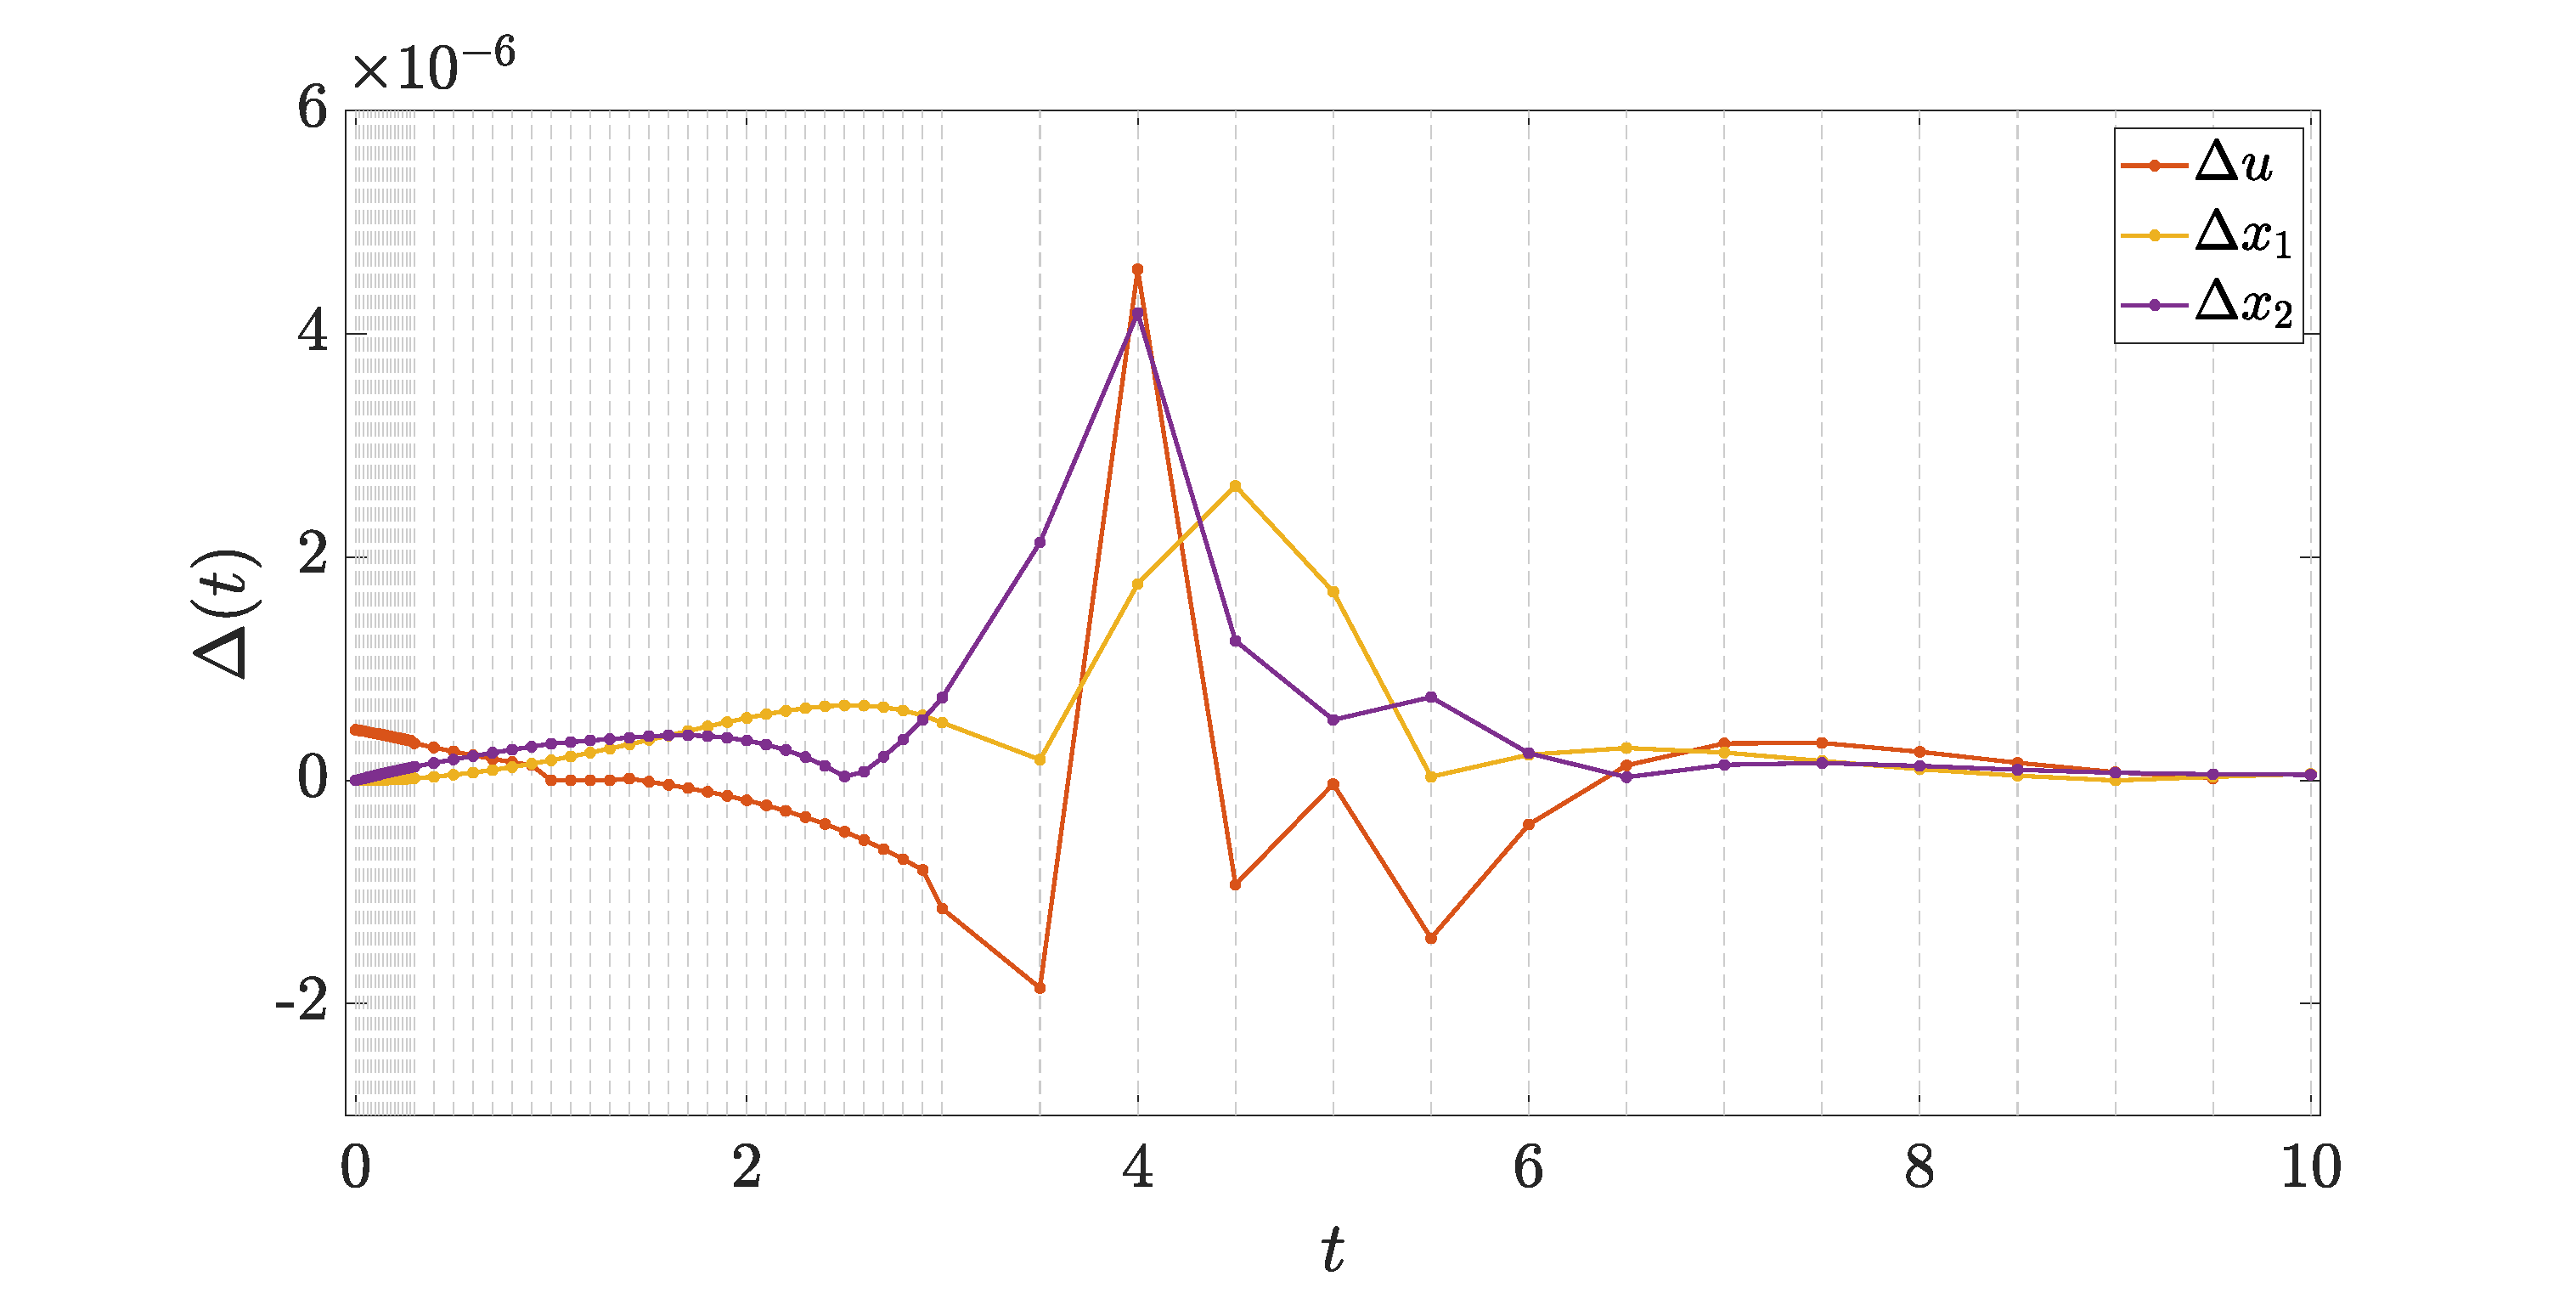
\includegraphics[trim={2cm 0cm 4cm 0cm},clip,width=1.\linewidth]{Img/delta_vanderpol}
	\caption{!!!!!}
	\label{fig:deltavanderpol}
\end{figure}



%%%%%%%%%%%%%%%%%%%%%%%%%%%%%%%%%%%%%%%%%%%%%%%%%%%%%%%%%%%%%%%%%%%%%%
\subsection*{Rolling Disk}
Esempio disco

%%%%%%%%%%%%%%%%%%%%%%%%%%%%%%%%%%%%%%%%%%%%%%%%%%%%%%%%%%%%%%%%%%%%%%
\subsection*{Free Flying Robot}
Esempio free flying robot

%\cite{latex, goosens} 


% Here's where you specify the bibliography style file.
% The full file name for the bibliography style file
% used for an ASME paper is asmems4.bst.
\bibliographystyle{asmems4}


%%%%%%%%%%%%%%%%%%%%%%%%%%%%%%%%%%%%%%%%%%%%%%%%%%%%%%%%%%%%%%%%%%%%%%
\section*{Conclusion}
prtova

%%%%%%%%%%%%%%%%%%%%%%%%%%%%%%%%%%%%%%%%%%%%%%%%%%%%%%%%%%%%%%%%%%%%%%

%\endgroup
\bibliography{marco}

%%%%%%%%%%%%%%%%%%%%%%%%%%%%%%%%%%%%%%%%%%%%%%%%%%%%%%%%%%%%%%%%%%%%%%
%\appendix       %%% starting appendix
%\section*{Appendix A: Head of First Appendix}
%Avoid Appendices if possible.

%%%%%%%%%%%%%%%%%%%%%%%%%%%%%%%%%%%%%%%%%%%%%%%%%%%%%%%%%%%%%%%%%%%%%%

\end{document}
